\section{Introduction}
\frame{\tableofcontents[currentsection, hideothersubsections]}

\begin{frame}
\frametitle{Introduction}

\begin{figure}
    \centering
    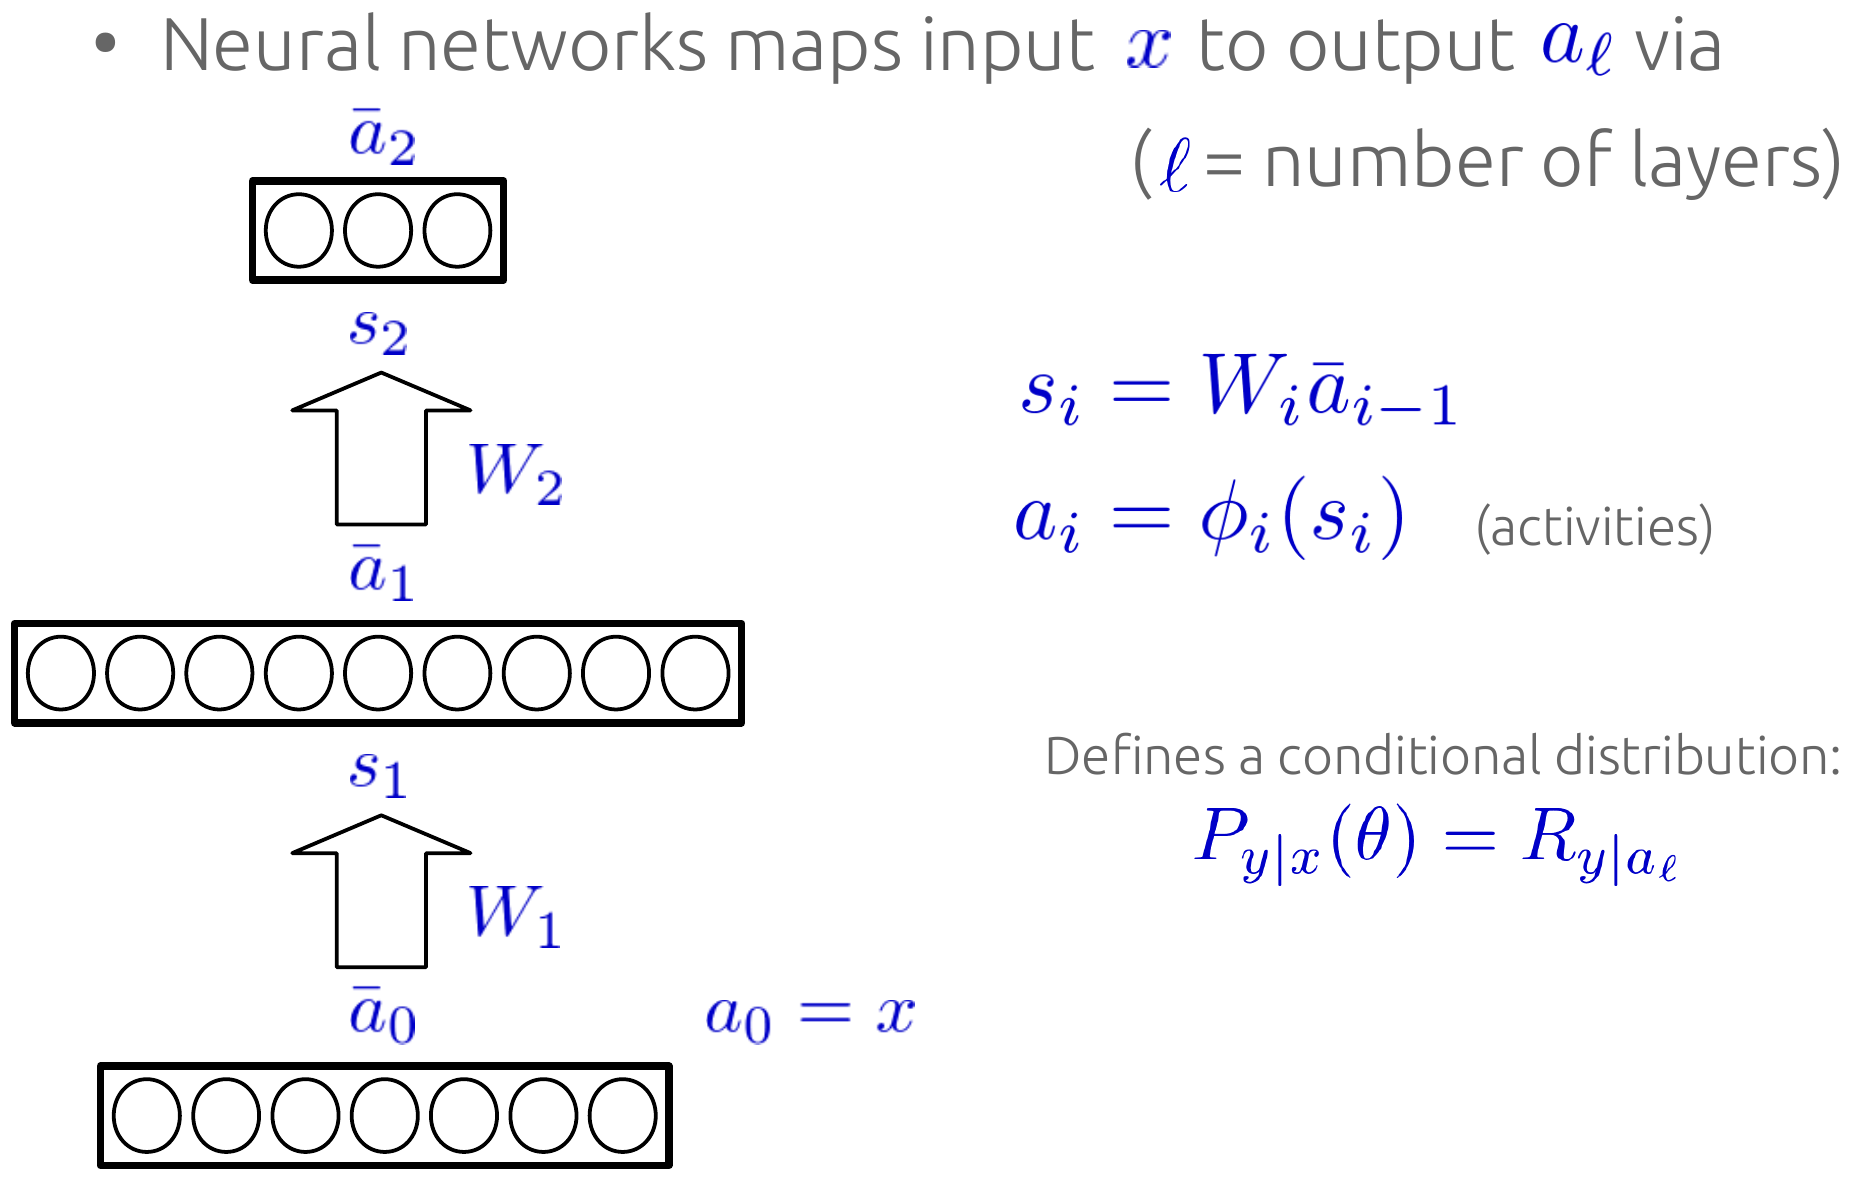
\includegraphics[scale=0.2]{net}
\end{figure}

{\footnotesize
\begin{itemize}
    \item $\bar{a}_i$ is $a_i$ appended by a homogeneous coordinate with value 1, ie
            to capture bias parameters explicitly
    \item $y$ is the target
\end{itemize}
}
\end{frame}

\begin{frame}
\frametitle{Introduction}

\begin{figure}
    \centering
    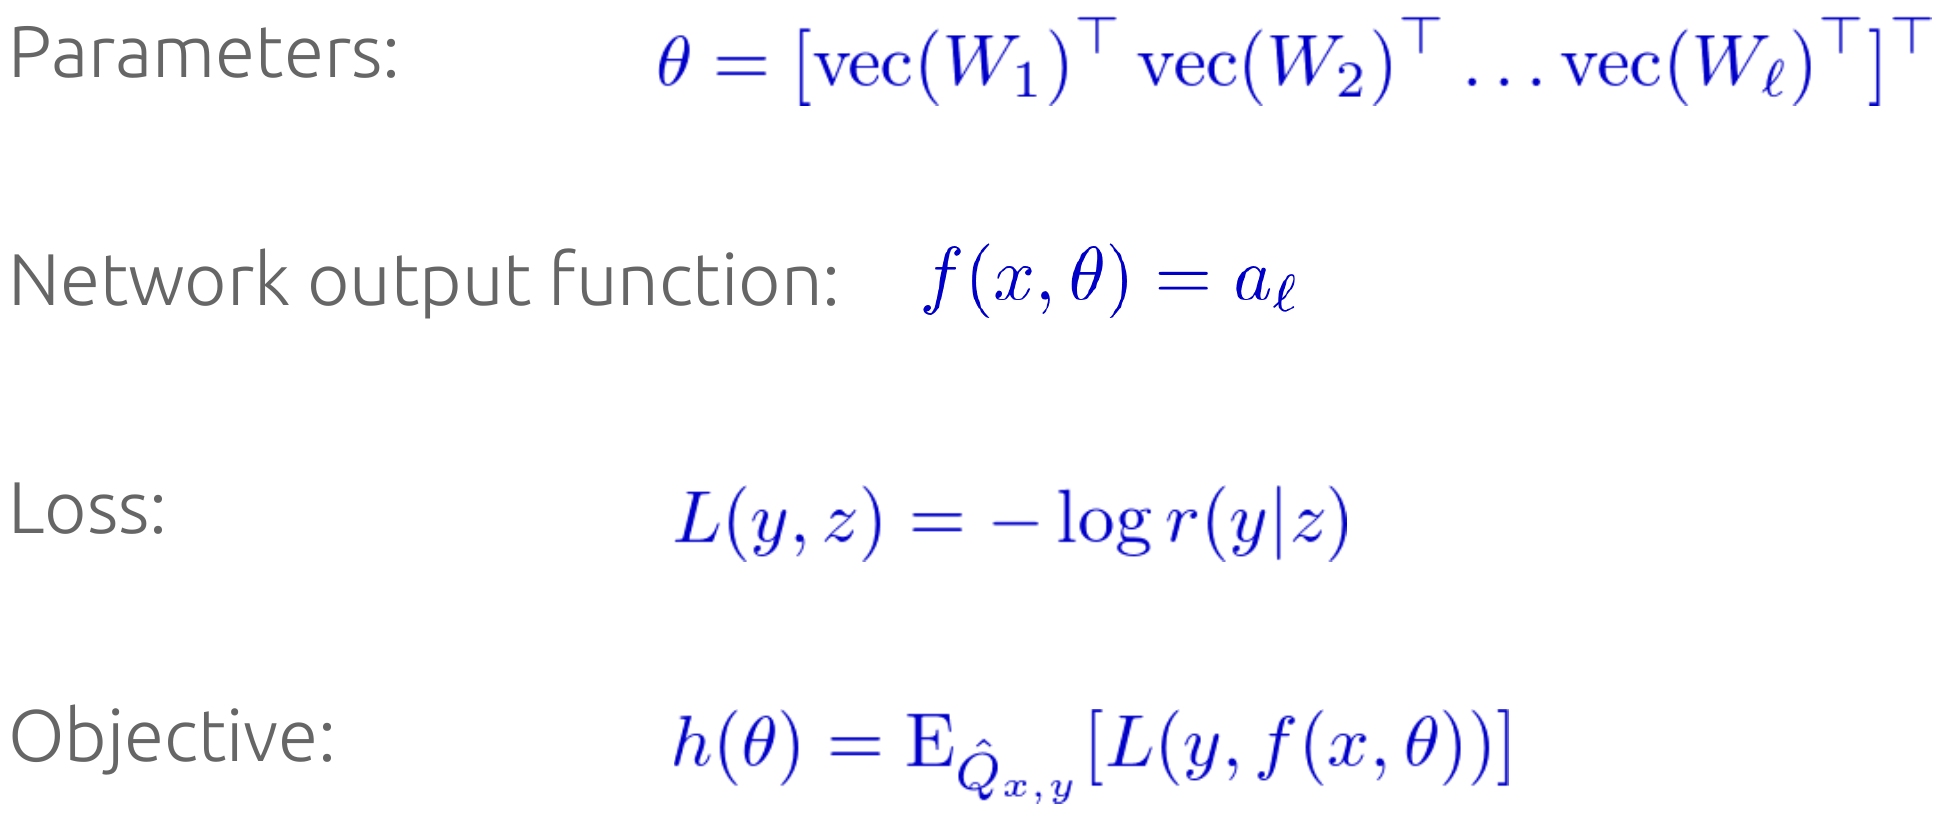
\includegraphics[scale=0.2]{net_param}
\end{figure}

{\footnotesize
\begin{itemize}
    \item $vec$ vectorizes matrices by stacking their columns together
    \item $\hat{Q}_{x, y}$ is a training distribution
    \item $p(y|x, \theta) = r(y|f(x, \theta))$ is the density function of $P_{y|x}(\theta) = R_{y|f(x,\theta)}$
    \item minimizing $h(\theta)$ can be seen as maximum likelihood learning of~$P_{y|x}(\theta)$.
\end{itemize}
}

\end{frame}

\begin{frame}
\frametitle{Introduction}
Newton-type update: $\theta_{k+1} = \theta_k - \alpha_k (\nabla^2 h)^{-1} \nabla h$
% \begin{itemize}
%     \item Newton-type update: $\theta_{t+1} = \theta_t - \alpha (\nabla^2 h)^{-1} \nabla h$
% \end{itemize}
\begin{figure}
    \raggedright
    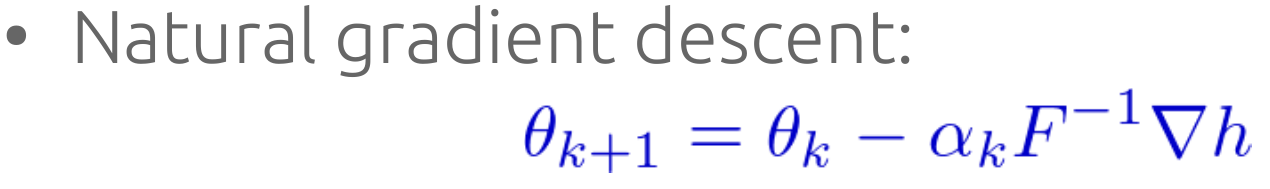
\includegraphics[scale=0.25]{natgrad}
\end{figure}

\begin{figure}
    \raggedright
    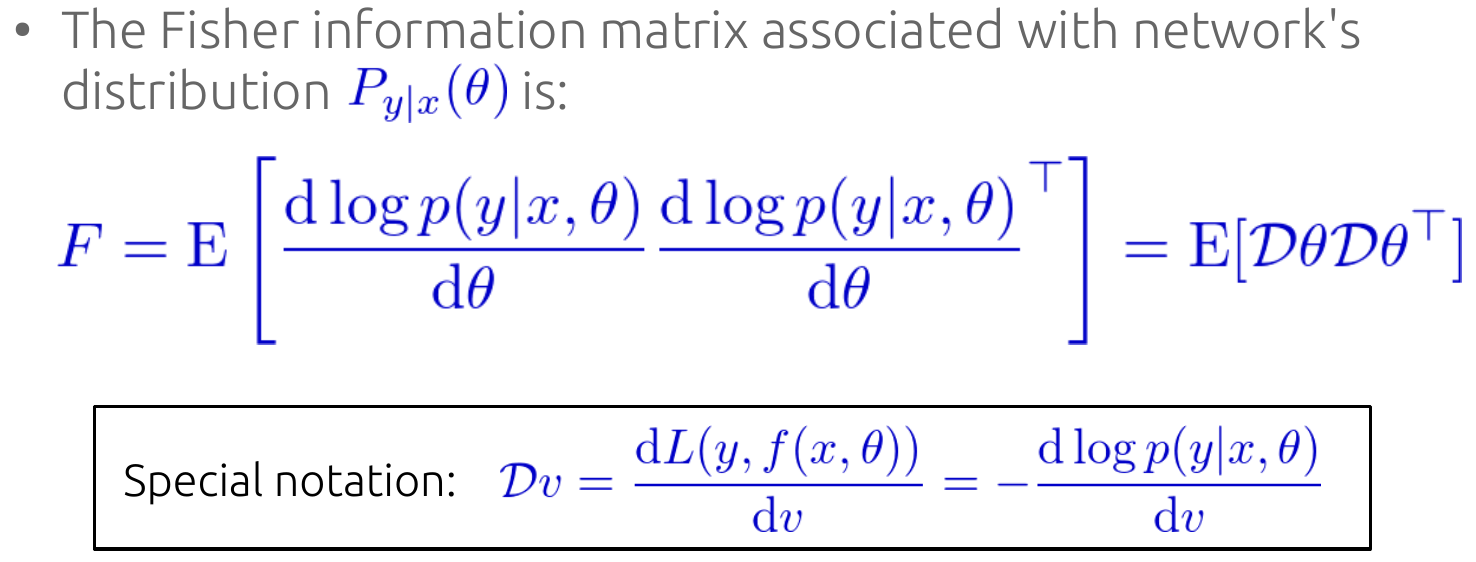
\includegraphics[scale=0.25]{fisher}
\end{figure}

{\footnotesize
\begin{itemize}
    \item can be viewed as the expected Hessian of loss under the model's distribution on $y$
    \item equals the generalized Gauss-Newton matrix used in HFO under certain conditions, \\
        see more on (Martens, 2014)
\end{itemize}
}

\end{frame}
